\section{Dense Reconstruction}

\emph{
  In applications such as 3D modelling, 3D printing, and AR/VR,
  a sparse model is not enough. When users are viewing the reconstruction,
  it is much more pleasing to deal with a dense reconstruction.
  To do this, it is helpful to rectify the images to make matching easier.
}
\subsection{Image Rectification}

\step
Initially, I would get an awkwardly-cropped
image when I tried to rectify the images.
I discovered that setting
the $M$ scaling factor passed to \verb|eight_point| to $1$
fixes the issue. The sparse projections looks unaffected,
but I saw other students mention on Slack that they ran into
the same issue.

\begin{figure}[H]
  \centering
  % minipage
  \begin{minipage}{.6\textwidth}
    \centering
    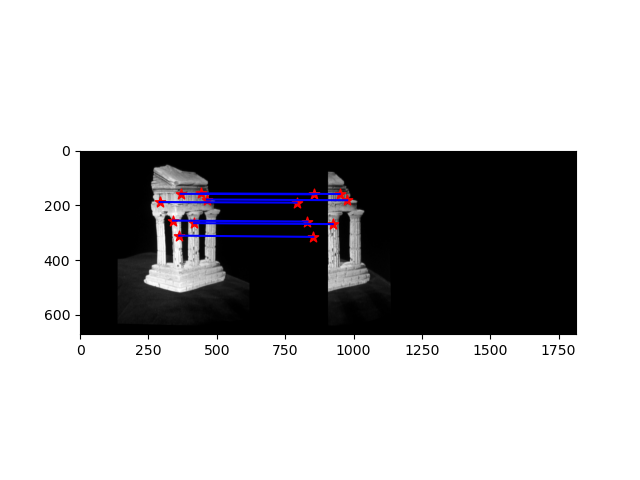
\includegraphics[width=\textwidth]{./figures/02-rectify-test-1.png}
    \caption{Dense Reconstruction, $M = \max(I_x, I_y)$}
  \end{minipage}
  \hfill
  % minipage
  \begin{minipage}{.6\textwidth}
    \centering
    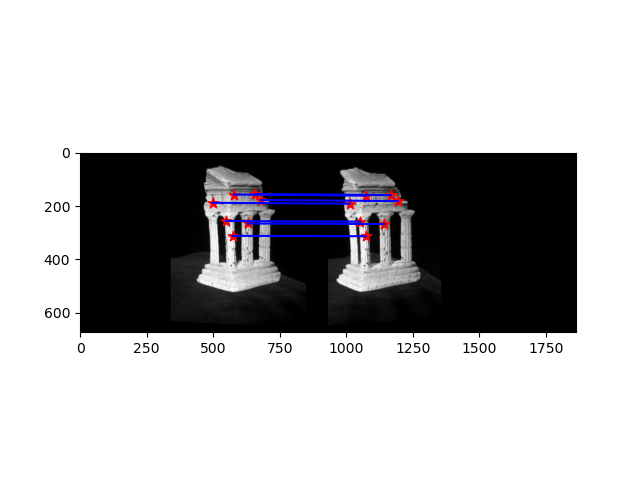
\includegraphics[width=\textwidth]{./figures/02-rectify-test-2.png}
    \caption{Dense Reconstruction, $M = 1$}
  \end{minipage}
\end{figure}

\newpage
\subsection{Disparity Map and Depth Map}

\step
Computed disparity and depth maps

\begin{figure}[H]
  \centering
  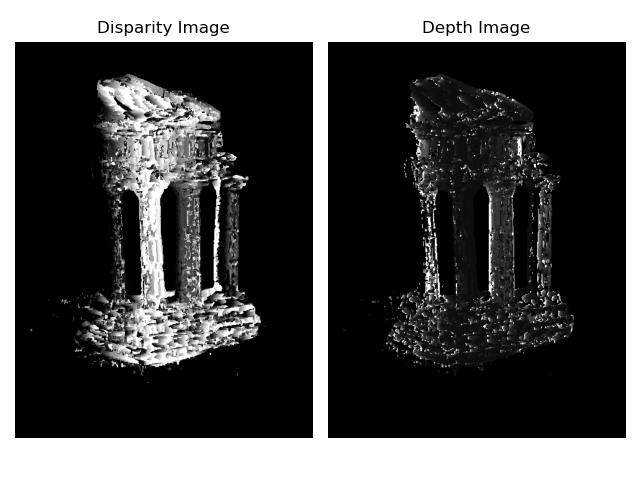
\includegraphics[width=\textwidth]{./figures/02-disparity+depth.png}
  \caption{Disparity and Depth Maps}  
\end{figure}
